%%%%%%%%%%%%%%%%%%%%%%%%%%%%%%%%%%%%%%%%%
%
% (c) 2018 by Jennifer Laaser
%
% This work is licensed under the Creative Commons Attribution-NonCommercial-ShareAlike 4.0 International License. To view a copy of this license, visit http://creativecommons.org/licenses/by-nc-sa/4.0/ or send a letter to Creative Commons, PO Box 1866, Mountain View, CA 94042, USA.
%
% The current source for these materials is accessible on Github: https://github.com/jlaaser/quantum-exercises
%
%%%%%%%%%%%%%%%%%%%%%%%%%%%%%%%%%%%%%%%%%

\section*{The Free Particle\sectionmark{Exercise: The Free Particle}}

Suppose a particle is traveling in a constant one-dimensional potential, $V(x)=V_c$.
	\begin{questions}
		\question What is the Hamiltonian for this particle?
				
					\vspace{0.1in}
					\begin{equation*}
						\hat H = \answerboxtall{125}
					\end{equation*}
					\vspace{0.1in}
				
		\question What is the Schr\"odinger equation for this particle?
				
					\vspace{0.1in}
					\begin{equation*}
						\answerboxtall{175} = E \Psi(x)
					\end{equation*}
					\vspace{0.1in}
				
		\question Try a solution of the form $\Psi(x) = e^{sx}$. What is $s$ in terms of the potential $V_c$, the particle's energy $E$, and the particle's mass, $m$?
					
					\begin{solution}[4.25in]
					\end{solution}
				
				\contdnewpg 
					
		\question If the particle's energy is greater than the potential, e.g. $E>V_c$, is $s$ real or imaginary?  Sketch the shape of the resulting wavefunction (or wavefunctions) on the graph below:
		
			\vspace{0.45in}
			\centerline{
				\begin{minipage}{0.5\textwidth}
				.
				\end{minipage}
				\begin{minipage}{0.4\textwidth}
					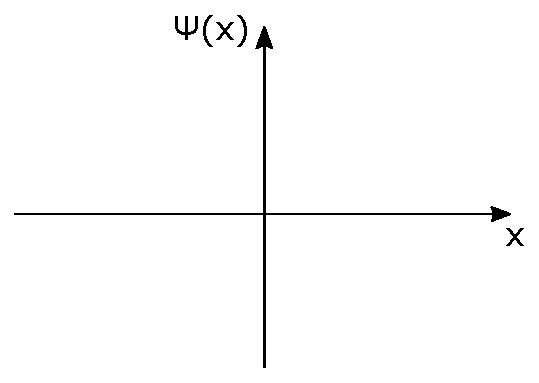
\includegraphics[width=\textwidth]{includes/free-particle-FIGURES/psi_axes.pdf}
				\end{minipage}
			}
			\vspace{0.45in}
				
		\question If the particle's energy is less than the potential, e.g. $E<V_c$, is $s$ real or imaginary?  Sketch the shape of the resulting wavefunction (or wavefunctions) on the graph below:
		
			\vspace{0.45in}
			\centerline{
				\begin{minipage}{0.5\textwidth}
				.
				\end{minipage}
				\begin{minipage}{0.4\textwidth}
					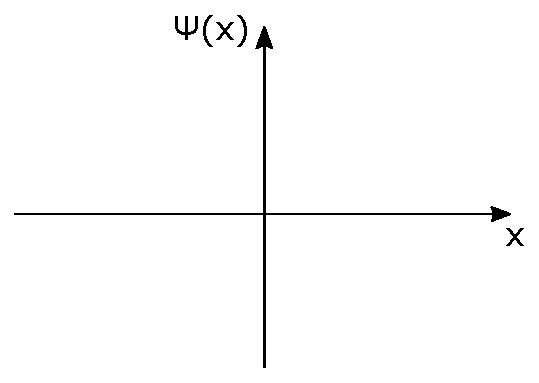
\includegraphics[width=\textwidth]{includes/free-particle-FIGURES/psi_axes.pdf}
				\end{minipage}
			}
			\vspace{0.45in}
				
		\question Why are the wavefunctions you found in questions 4 and 5 difficult to normalize?
		
			\begin{solution}[1.75in]
			\end{solution}
	\end{questions}
	
\stophere